\section{Computational model}

        Il modello migliore è stato ottenuto dopo una prima fase di \textit{data preparation}, ed una successiva fase di \textit{hyper-parameter tuning}.

        \subsection{Data preparation}
        
                \subsubsection{Data splitting}
                
                        Il dataset è stato diviso in due sezioni differenti:
                        \begin{itemize}
                                \item training set: contiene 80\% dell'intero dataset originale (6400 records)
                                \item test set: contiene il restante 20\% del dataset originale (1600 records)
                        \end{itemize}
                
                \subsubsection{Missing data management}
                
                        Il dataset originale contiene dati mancanti in corrispondenza di alcune delle features, per questo motivo, i valori relativi a tali campi sono stati sostituiti con il valore medio della feature all'interno del dataset.
                
                \subsubsection{Outlier management}
                
                        Per la gestione degli \textit{outlier} del dataset sono stati analizzati i risultati derivanti da tre metodi:
                        \begin{itemize}
                                \item \textit{z-score}
                                \item \textit{modified z-score}
                                \item \textit{inter-quantile range}
                        \end{itemize}
                    
                        \textbf{TODO - descrivere in formule gli approcci dei 3 metodi}
                
                \subsubsection{Data scaling}
                
                \subsubsection{Feature selection}
                
                        In questa fase sono state selezionate le \textit{features} più significative al fine di ridurre i costi di training e migliorare la capacità di generalizzazione del classificatore.
                        
                        Pair plot:
                        \begin{figure}[!h]
                            \centering
                            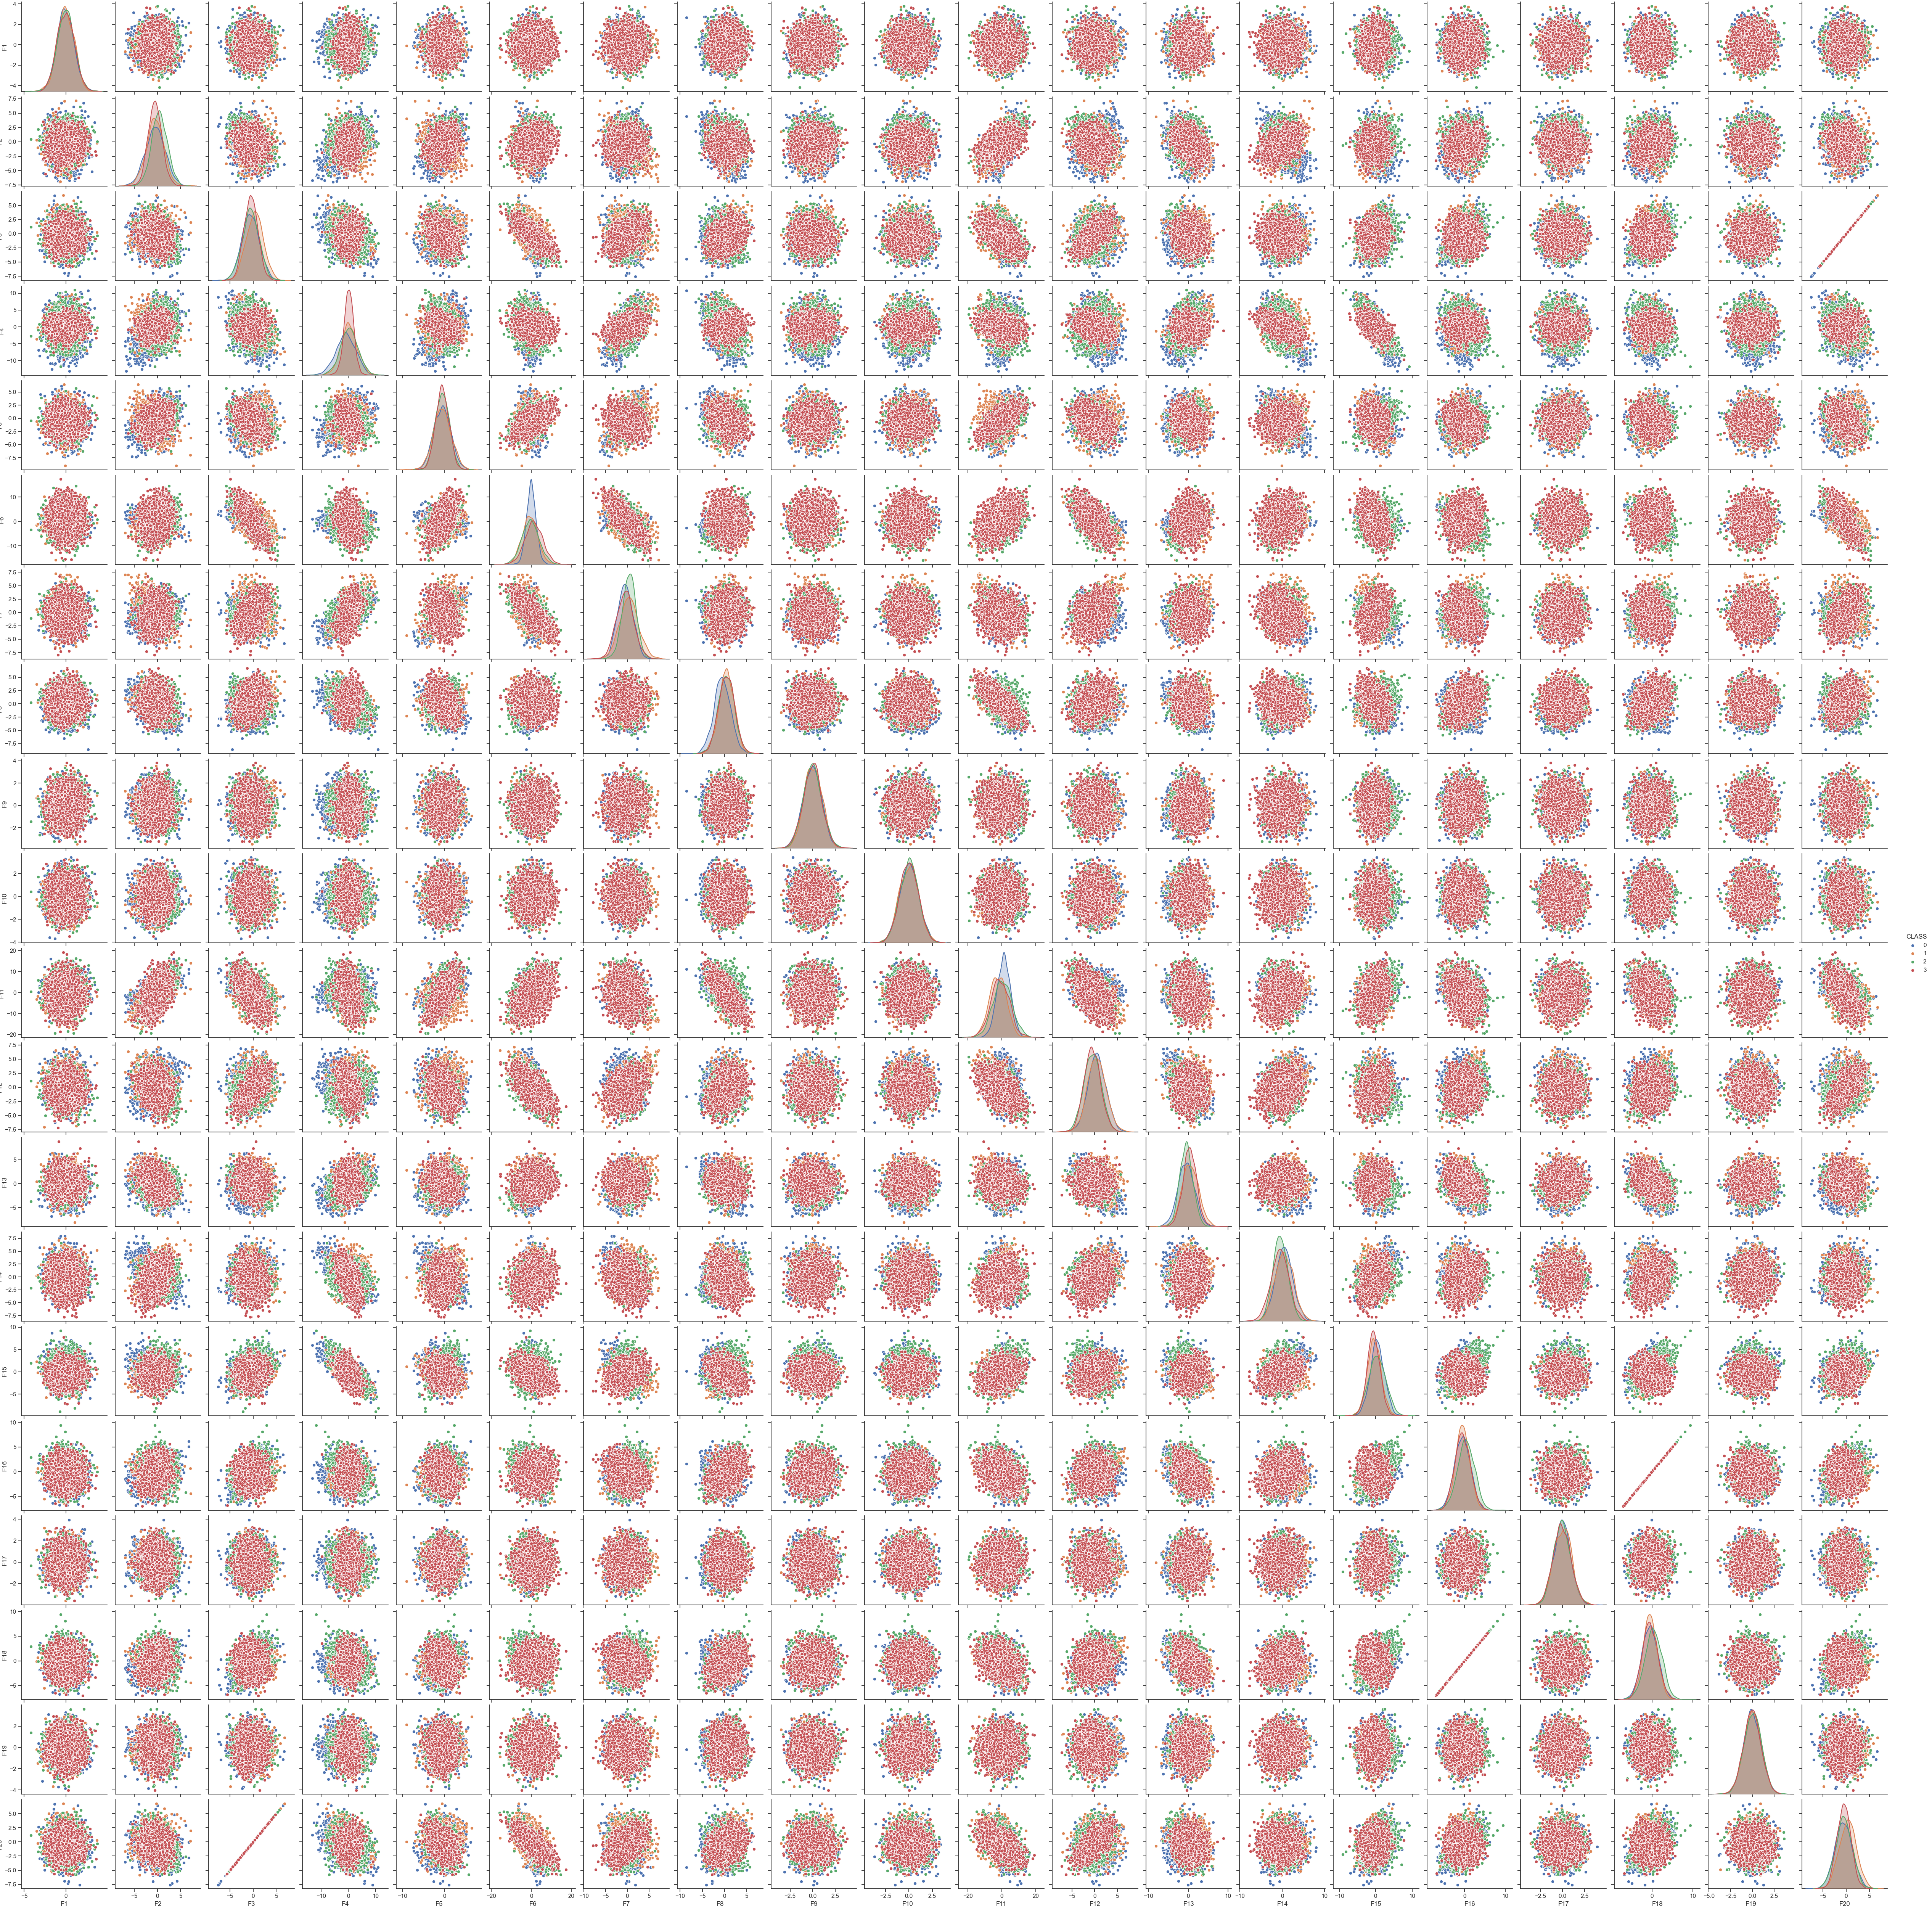
\includegraphics[width=175mm]{training_set}
                            \caption{Pair plot representing \textit{features}.}
                            \label{fig:training_set_pairplot}
                        \end{figure}
                
                \subsubsection{Data sampling}  
                
                

        \subsection{Hyper-parameters tuning}
        
                In questa fase sono stati cercati gli \textit{iper-parametri} per i vari classificatori.